In Year 2, we focused on advancing magnetohydrodynamic (MHD) capabilities to support high-fidelity modeling of liquid-metal blankets. Our primary target was the ITER Water-Cooled Lead-Lithium (WCLL) blanket—a leading breeding blanket concept that combines tritium breeding in PbLi with active water cooling. This configuration represents a canonical exascale multiphysics challenge, requiring the coupling of liquid-metal flows, heat transfer, MHD, neutron transport, and structural mechanics.

We performed unprecedented high-resolution simulations of the WCLL blanket using the GPU-accelerated code \texttt{NekRS}, building upon developments from the ExaSMR project under the DOE Exascale Computing Project (ECP). \texttt{NekRS} demonstrated exceptional scalability and performance on Frontier and Aurora. A major effort this year was the development of a robust, GPU-based MHD solver and its initial validation against analytical benchmarks (Figure~\ref{fig:thanh}).

\begin{figure}[h]
\centering
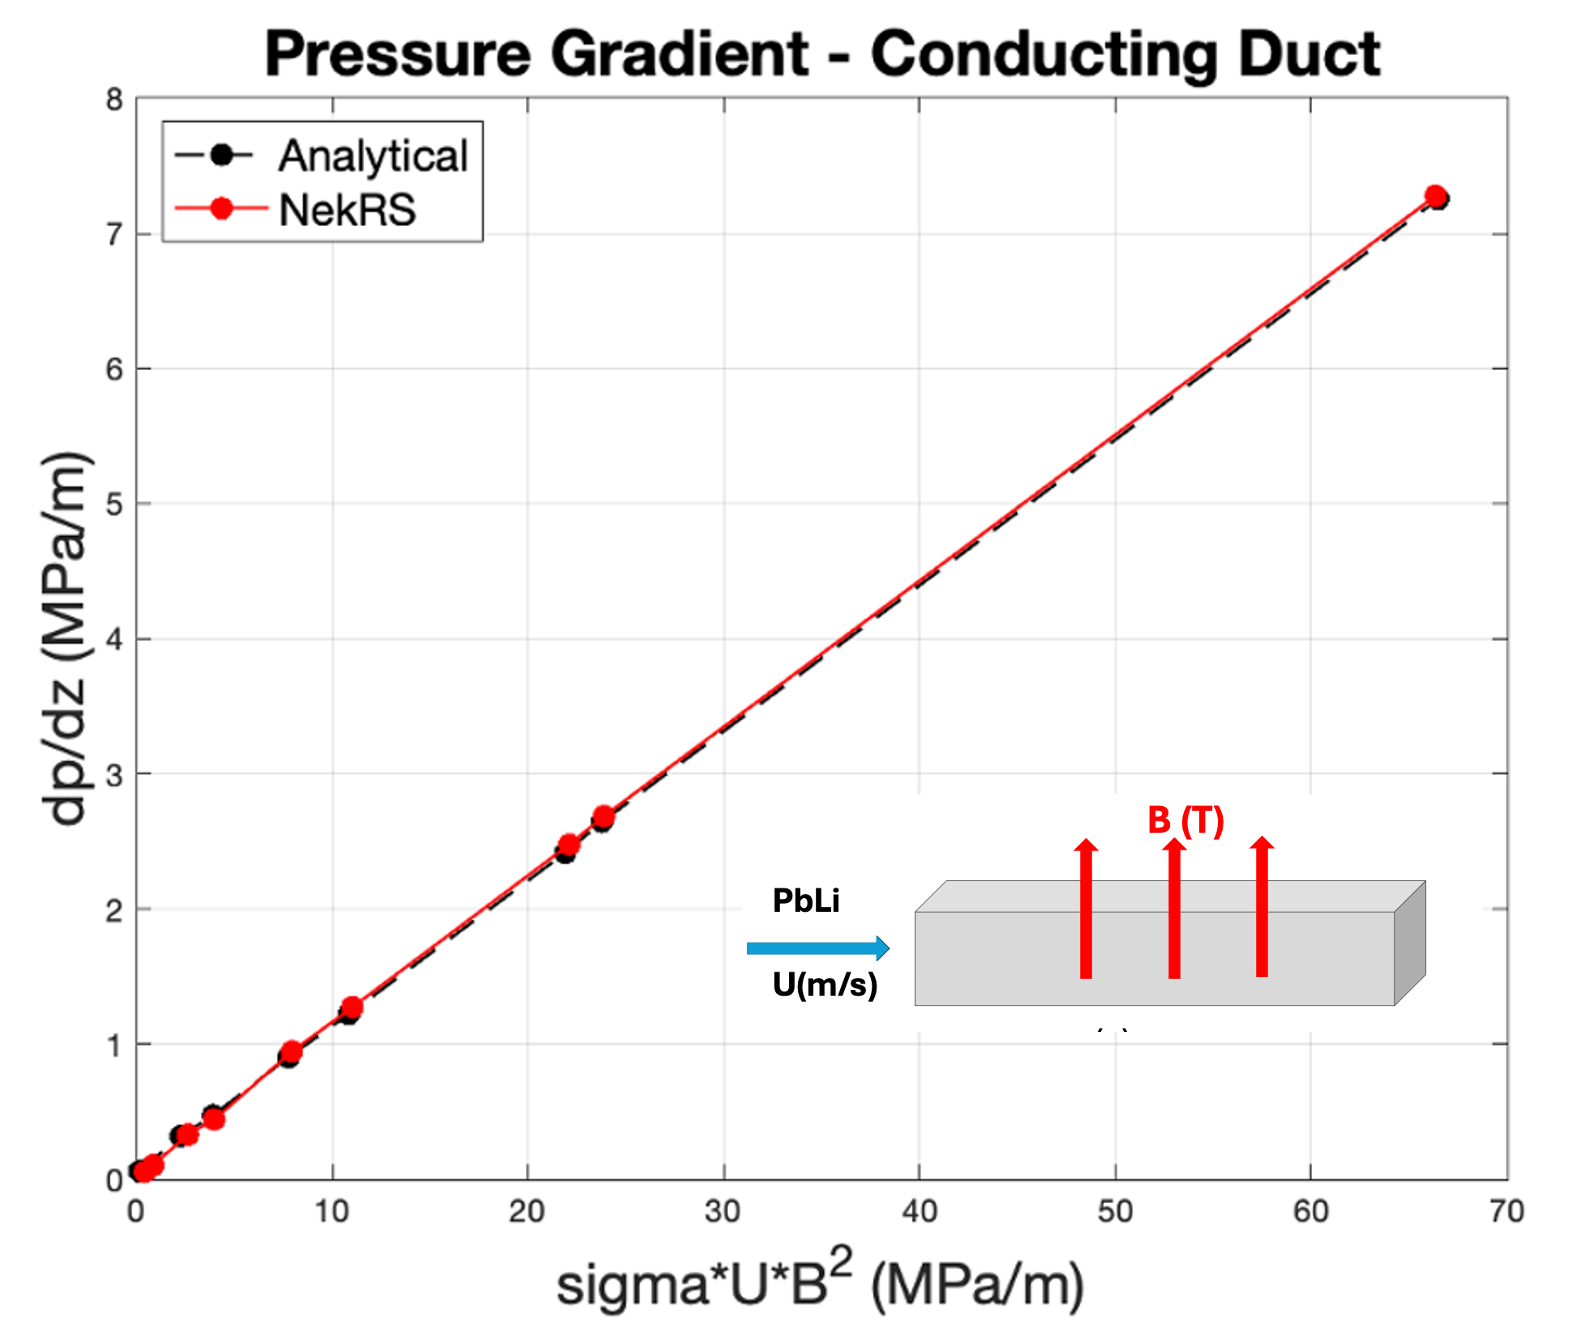
\includegraphics[width=2.5in]{figs/thanh_case.png}
\caption{\label{fig:thanh} Validation of PbLi MHD pressure gradients with analytical predictions.}
\end{figure}

We then carried out a series of large-scale simulations:

\begin{enumerate}
\item \textbf{Lead-Lithium Simulations:} These simulations used up to $1.9$ billion spectral elements (equivalent to $6.6\times 10^{11}$ gridpoints at polynomial order $N=7$) to resolve wall-bounded turbulent flow under strong magnetic fields ($Ha \sim 10^4$). This constitutes the largest liquid-metal MHD simulation conducted to date. Volumetric heat sources and tritium generation rates were obtained from \texttt{OpenMC} transport calculations. Magnetic induction effects were fully coupled across fluid and solid conducting regions.

\item \textbf{Water Cooling System:} Simulations of the high-Reynolds-number water cooling loop were performed using comparable mesh sizes with boundary layer-resolving resolution. These runs validated both model fidelity and scalability across thousands of GPU nodes.
\end{enumerate}

We emphasize that this work represents the first full-scale, coupled liquid-metal MHD and thermal simulations of the WCLL blanket, resolving nearly one trillion degrees of freedom across the PbLi and water domains. The simulations leverage high-order spectral element methods, matrix-free GPU kernels, scalable \$p\$-multigrid solvers, and reuse of geometric factors for computational efficiency. Results reveal that MHD significantly alters flow fields and turbulence structure, with important engineering consequences for pressure drop, heat transfer, and tritium breeding performance (Figs. \ref{fig:sec5}, \ref{fig:sec5a}). Our goal is to establish the ability to resolve coupled LM-MHD and thermal behavior at reactor scale, informed by nuclear transport calculations, thereby enabling virtual qualification of breeding blanket designs. Once validated, these tools will support rapid design iteration, complement experimental efforts, and accelerate the pathway to commercial fusion energy.

\begin{figure}[h]
\centering
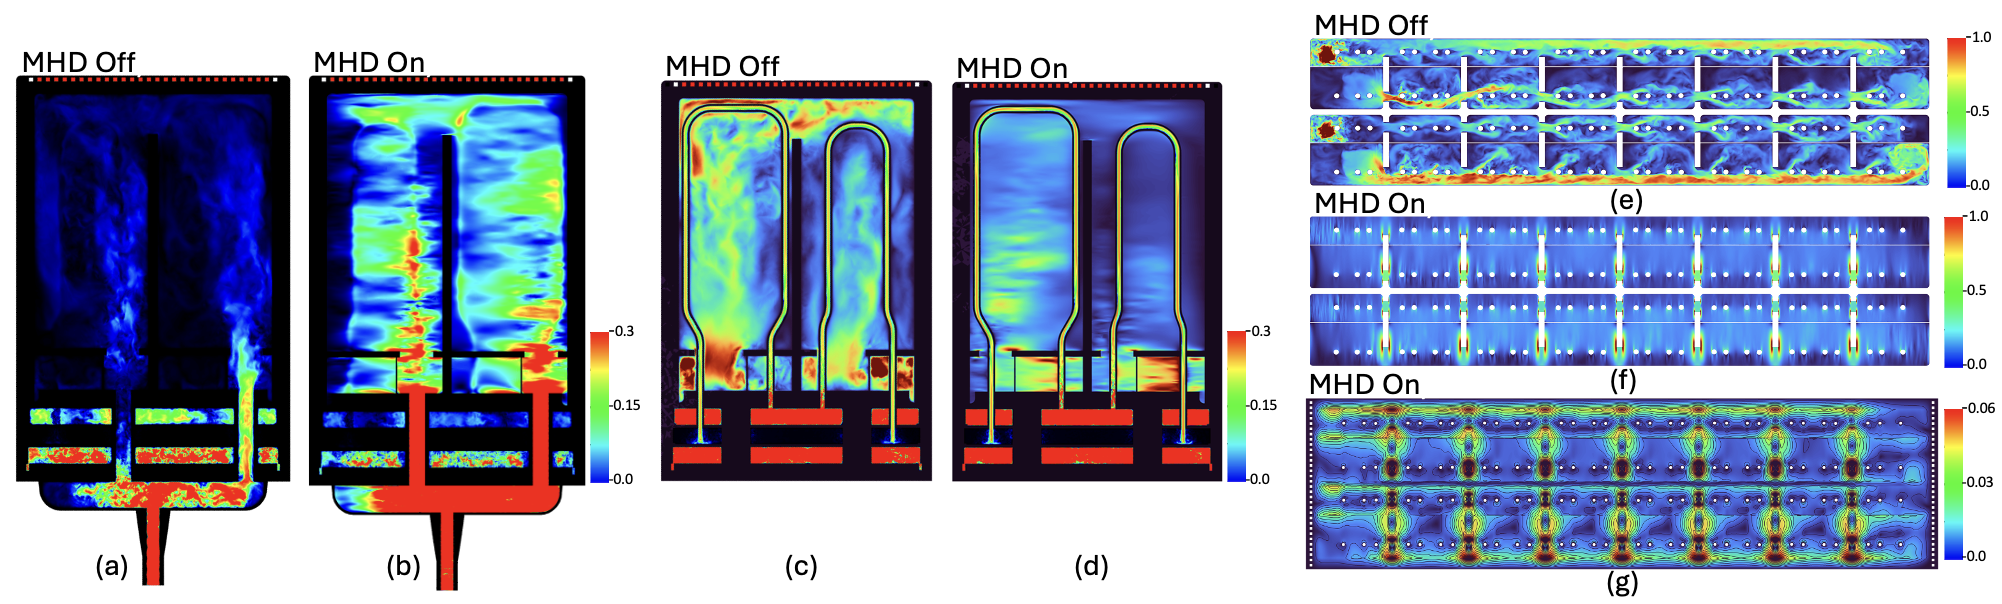
\includegraphics[width=6.0in]{figs/mhd_onoff_a2g_2.png}
\caption{\label{fig:sec5}
Impact of MHD on PbLi flow: (a, c, e) without magnetic field; (b, d, f) with magnetic field; (g) magnetic field strength. Water cooling loops are shown in (c, d).
}
\end{figure}

\begin{figure}[h]
\centering
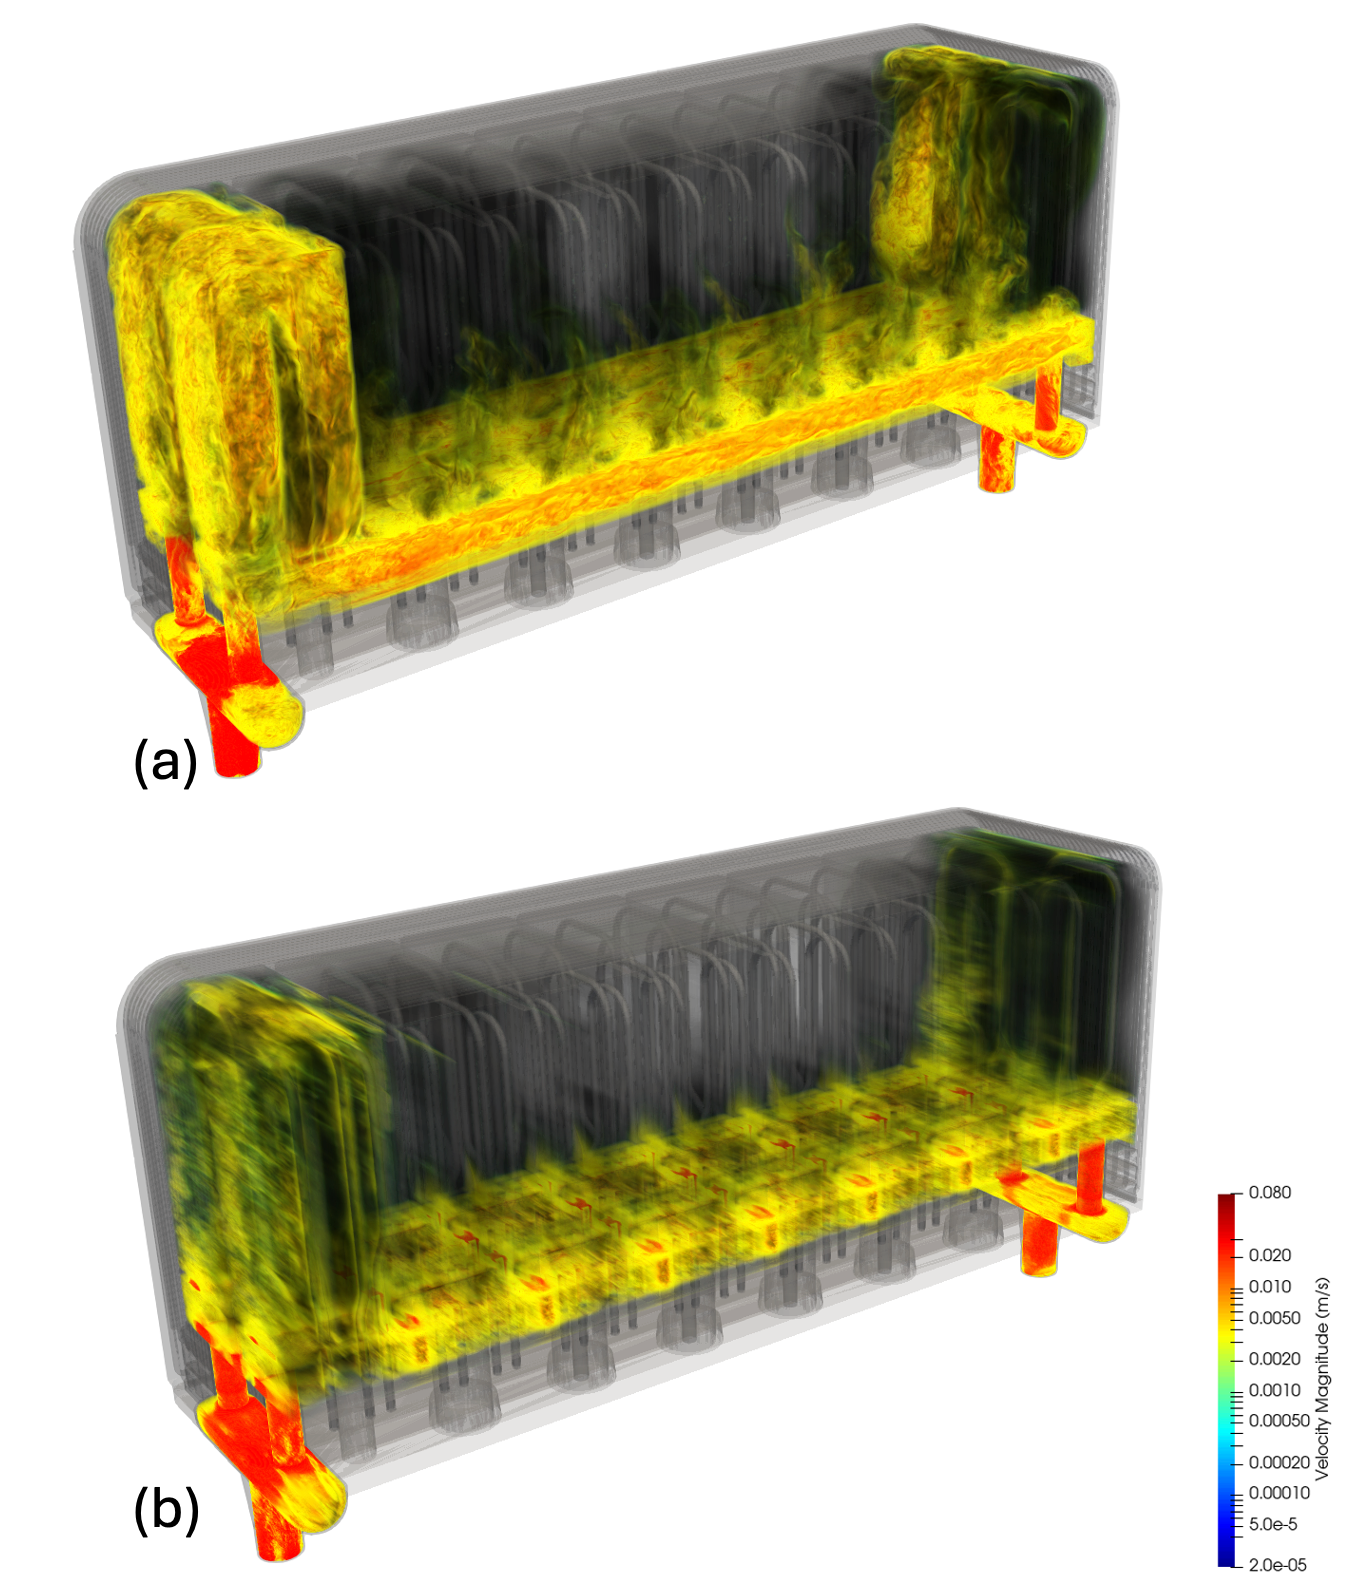
\includegraphics[width=2.0in]{figs/volume_PbLi_index_logv_vert.png}
\caption{\label{fig:sec5a}
Volume rendering of PbLi velocity with and without MHD. Anisotropic turbulence suppression due to the magnetic field is clearly visible.
}
\end{figure}

%
%===


